
%(BEGIN_QUESTION)
% Copyright 2015, Tony R. Kuphaldt, released under the Creative Commons Attribution License (v 1.0)
% This means you may do almost anything with this work of mine, so long as you give me proper credit

Rotasjonsretningen til en trefase AC-motor kan reverseres ved å bytte om på hvilke som helst to av de tre faseledertilkoblingene. Med dette i bakhodet: Forklar hvordan denne reverserende motorstyringskretsen fungerer:

$$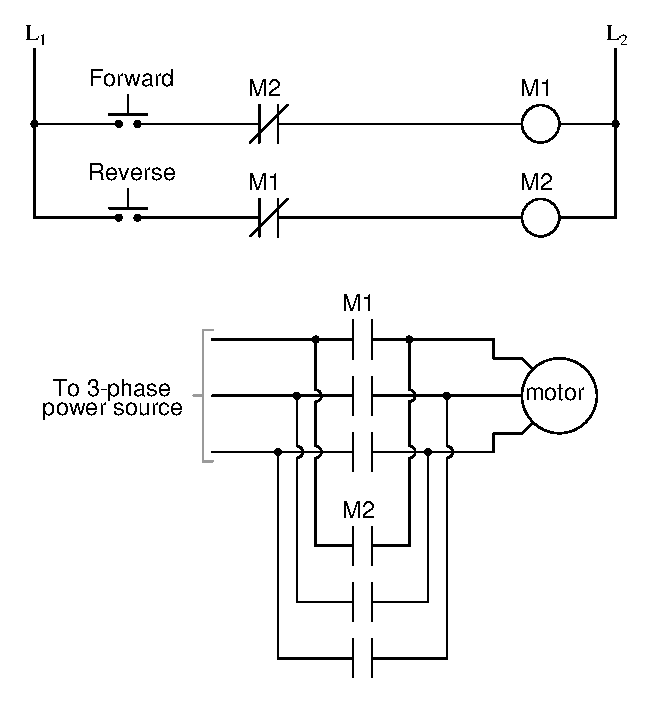
\includegraphics[width=15.5cm]{i01391x01.eps}$$

Forklar særlig funksjonen til de to normalt lukkede ``M''-kontaktene (kalt {\it forriglingskontakter}) i styrekretsen. Hva tror du kan skje dersom disse kontaktene ikke var der?

\vskip 20pt \vbox{\hrule \hbox{\strut \vrule{} {\bf Forslag til sokratisk diskusjon} \vrule} \hrule}

\begin{itemize}
\item{} Forklar {\it hvorfor} det å bytte om to faseledere i AC-forsyningen til en induksjonsmotor får den til å skifte rotasjonsretning.
\item{} Forklar hva {\it arc flash} (lysbueulykke) er, og hvordan du beskytter deg mot dette når du arbeider på høyspente motorstyringskretser som denne.
\item{} Anta at en elektriker prøver å tvinge motoren til å gå i foroverretning ved å koble en midlertidig lask over reléspolen M1. Oppnår han ønsket resultat? Forklar hvorfor eller hvorfor ikke, og identifiser også eventuelle sikkerhetsfarer ved å gjøre dette.
\item{} Anta at en elektriker prøver å tvinge motoren til å gå i foroverretning ved å koble en midlertidig lask over ``Forward''-trykknappen. Oppnår han ønsket resultat? Forklar hvorfor eller hvorfor ikke, og identifiser også eventuelle sikkerhetsfarer ved å gjøre dette.
\item{} Anta at en elektriker prøver å tvinge motoren til å gå i foroverretning ved å koble tre midlertidige lasker over M1-kontaktene. Oppnår han ønsket resultat? Forklar hvorfor eller hvorfor ikke, og identifiser også eventuelle sikkerhetsfarer ved å gjøre dette.
\end{itemize}

\underbar{file i01391}
%(END_QUESTION)





%(BEGIN_ANSWER)

De normalt lukkede kontaktene kalles {\it forriglingskontakter}, og de hindrer samtidig innkobling av motorens {\it forover}- og {\it revers}-retning.
 
%(END_ANSWER)





%(BEGIN_NOTES)

Selvsagt: Hvis både forover- og revers-kontaktorene noen gang skulle trekke samtidig, blir resultatet en direkte fase-til-fase-kortslutning!







\vfil \eject

\noindent
{\bf Oppsummeringsquiz:}

Forklar i detalj hvilken funksjon {\it forriglingskontakter} har i en motorstyringskrets. Bruk gjerne et praktisk eksempel dersom det hjelper forklaringen din.

%INDEX% Final Control Elements, valve: electric actuator

%(END_NOTES)

